\documentclass[11pt]{article}
\usepackage[utf8]{inputenc}
\usepackage[T1]{fontenc}
\usepackage{minted}
\usepackage{graphicx}
\usepackage{hyperref}
\usepackage{CJKutf8}

\author{Student: Brian Cheung bc32427 \\ Professor: Mohit Tiwari \\ TA: Antonio Espinoza \\ Department of Electrical \& Computer Engineering \\ The University of Texas at Austin}
\date{\today}
\title{EE379K Enterprise Network Security Lab 3 Report}
\hypersetup{
 pdfauthor={Student: Brian Cheung bc32427 \\ Professor: Mohit Tiwari \\ TA: Antonio Espinoza \\ Department of Electrical \& Computer Engineering \\ The University of Texas at Austin},
 pdftitle={EE379K Enterprise Network Security Lab 3 Report},
 pdfkeywords={},
 pdfsubject={},
 pdfcreator={},
 pdflang={English}}

\begin{document}

\maketitle
\newpage
\section*{Part 1 - APT Campaign Questions}
\label{sec:part-1}

\subsection*{Exercise Set 1}
\begin{enumerate}
  \item Dwell time is the number of days from when an attacker first compromises
  the victim to when the attacker is finally detected. The decrease in median dwell
  time over the past year can be attributed to the improvement of "internal hunting
  capabilities" and "enhanced network, endpoint and cloud-service provider visibility."~\cite{m-trend}
  \item Advanced Persistent Threat (APT) groups are "generally focused on espionage activities."
  \begin{itemize}
    \item APT37 ("Reaper") - Active since 2012, APT37 primarily targets organizations
    in South Korea, but have recently started targeting Japan, Vietnam, and the
    Middle East in order to gain intelligence for North Korea's military, political,
    and economic interests.
    \item APT38 - APT38 uses destructive malware to steal hundreds of millions of dollars
    from financial institutions. This group is linked to North Korean espionage operators.
    \item APT39 - APT 39 is an Iranian cyber espionage group primarily targeting the Middle East.
    It targets the telecommunications sector, travel industry and supporting IT firms,
    and the high-tech industry in order to monitor and track specific individuals and collect
    customer data for strategic purposes related to national priorities.
    \item APT40 ("Periscope") - APT40 is a Chinese espionage group that targets Southeast
    Asian countries that are important to China's "Belt and Road Initiative". The group takes
    large amounts of information from organizations in the engineering, transportation,
    and defense sectors related to maritime technologies.
  \end{itemize}
  \item The known methods of initial compromise for APT37 include phishing operations
  and strategic web compromise.
  Specifically, APT37 sent a reunification-themed email that contained a weaponized HWP attachment.
  This spearphishing attachment is a form of social engineering that relies on the victim
  to execute the attachment which compromises the victim's system. "Network intrusion detection
  systems and email gateways can be used to detect spearphishing with malicious attachments."~\cite{phishing}
  APT37 also used social networking and cloud platforms like Twitter, AOL, and Dropbox to relay
  commands to compromise the victim's systems. Analyzing network data for abnormal data flows and
  unexpected protocol behaviors may be useful in detecting such attacks.~\cite{web-service}
  \item A lack of investigation on infected systems may cause the victim to overlook the
  the possibility of a larger breach. After detection of malware on a system, it is important
  to understand that the piece of malware may have stemmed from a lateral movement from
  another system in the environment, and not just a new isolated attack. This understanding would
  encourage the victim to run a more thorough investigation to detect the breach.
  A poorly timed remediation may actually hurt the victim even further. If an attacker has had
  long term access to the victim, the attacker may likely have many different ways to evade eradication
  methods. As a result of a poorly time remediation, the victim could fail to eradicate the attacker
  and even complicate the investigation further prolonging the investigation and remediation process.
  This mistake can be avoided by conducting regular reviews of incident response plans, use cases,
  and playbooks in addition to properly handling and storing evidence in incident respons plans.
  Organizations should also develop guidelines and procedures for analyzing threats ion addition to
  erradication and remediation plans.
\end{enumerate}
\subsection*{Exercise Set 2}
\begin{enumerate}
  \setcounter{enumi}{4}
  \item According to MITRE~\cite{web-service}, the Web Service attack is a Command and Control
  and Defense Evasion tactic. Since this attack often uses common services that the victim
  is already using and web service providers often us SSL/TSL encryption, attackers can easily hide
  under the "expected noise" and extra level of protection.
  \item Web services commonly used in a Web Service attack:~\ref{table:web-services}
  \begin{table}[h]
    \centering
    \begin{tabular}{ |c|c| }
      \hline
      \textbf{Web Service} & \textbf{Examples} \\
      \hline
      Social Networking & 10  \\
      Cloud Storage     & 9   \\
      Github            & 7   \\
      Google Services   & 7   \\
      Pastebin          & 5   \\
      Blogs             & 3   \\
      Downloader        & 1   \\
      \hline
    \end{tabular}
    \caption{\label{table:web-services}
    Table of web services commonly used in a Web Service attack.}
  \end{table}
  \item Social networking platforms like Twitter, cloud storage services like Dropbox,
  and Github are often used in a Web Service attack. These services allow attackers
  to post content embedded with malicious domains or IP addresses that infect victims.
  A victim may be able to detect the malicious intent through abnormal data flows
  and suspicious activity when accessing content on these services.
\end{enumerate}

\subsection*{Exercise Set 3}
\begin{enumerate}
  \setcounter{enumi}{7}
  \item APT41 targets the video game industry by "stealing source code and digital
  certificates, virtual currency manipulation, and attempting to deploy ransomware."~\cite{apt41}
  An APT group like APT41 could be interested in targeting the video game industry
  for financial gains.
  \item APT29 is a Russian cyber threat group that has a very sophisticated way of communicating
  with the malware, Hammertoss.~\cite{apt29}
  \begin{enumerate}
    \item The malware generates a Twitter handle (user ID) based on the specific day.
    This tells the malware which Twitter account to check for a tweet that contains
    instructions for the next stage in the process. If the Twitter account isn't registered,
    then Hammertoss will wait for the next day to begin the process again.
    \item If APT29 registered the specific Twitter account for that day, the group
    will tweet a URL that directs Hammertoss to a webpage that contains images along
    with a hashtag that specifies the offset of the hidden data and the characters for decryption.
    \item For example, the URL can link to a Github page where APT29 has uploaded an image
    appended with encrypted data. Hammertoss will visit this page and download the image.
    \item Hammertoss then decrypts the data with the instructions specified in the tweet.
    \item The data may include commands or login credentials that instructs Hammertoss
    to upload a victim's data to a cloud storage service. Once uploaded, APT29 can
    retrieve the information.
  \end{enumerate}
  APT29 makes the process difficult to detect by using Twitter as an extra layer of obfuscation.
  Additionally, APT29 registers only a small number of accounts and only communicates at certain
  times keeping their footprint small and indistinguishable from normal traffic.
  \item Sudo prompts the user for the password and allows the user to run commands with
  root privelages. It can also cache the credentials by storing the timestamp of when
  \verb|sudo| was last run. This allows the user to have root privelages for a certain period of time.
  This caching is isolated to a specific terminal session with the \verb|tty_tickets| variable.
  However, this can be abused to allow malware to execute commands with elevated privelages without
  the user's password by seeing if timestamps  fall within the timeout range. If \verb|tty_tickets|
  are disables, the malware can do this from any terminal session for the user. This can be detected
  by monitoring the I/O logs from the \verb|/etc/sudoers| file. To stop such acttacks,
  the user needs to ensure the \verb|tty_tickets| setting is enabled to prevent any leakage across
  terminal sessions. Users can also set the \verb|timestamp_timeout| to 0 which would require the
  user to input their password each time \verb|sudo| is executed.~\cite{sudo-caching}
  \item MimiPenguin uses a technique called Credential Dumping.~\cite{mimipenguin}
  This technique is a form of Credential Access that involves dumping process memory and
  extracting clear-text credentials.~\cite{credential-dumping}
\end{enumerate}

\section*{Part 2 - Fuzzing}
\label{sec:part-2}

\begin{enumerate}
  \item The Vulnserver expects a command followed by an argument. If an invalid command is sent or
  no argument is provided, then the server responds with "UNKOWN COMMAND". The fuzzer (part-2/fuzzer.py) generates
  a random string for a random command and keeps increasing the length of the string until it observes
  unexpected behavior. Then it changes to a different command and repeats until the Vulnserver crashes.
  The fuzzer also creates two output files in the output directory (part-2/output/). The \verb|success.txt| file
  logs all of the successful commands that didn't cause any unexpected behavior. The \verb|failure.txt|
  file logs all of the commands that caused unexpected behavior. After running the fuzzer
  and analyzing the output files, the \verb|failure.txt| file shows that a string length of at least 4110
  caused unexpected behavior. Sometimes the server crashes and sometimes the server responded with
  "UNKOWN COMMAND" followed by some additional responses even for a known command. After causing buffer overflow,
  sending a different command seems to crash the Vulnserver as well.
  \item The extremely long string caused the buffer to overflow which caused unexpected behavior.
  The buffer overflow could be exploited to execute shellcode.
\end{enumerate}

\section*{Part 3 - Exploitation}
\label{sec:part-3}

\begin{enumerate}
  \item The exploit uses HTTP to communicate with the application as shown in Figure~\ref{fig:wireshark-http}.
  \begin{figure}[htbp]
    \centering
    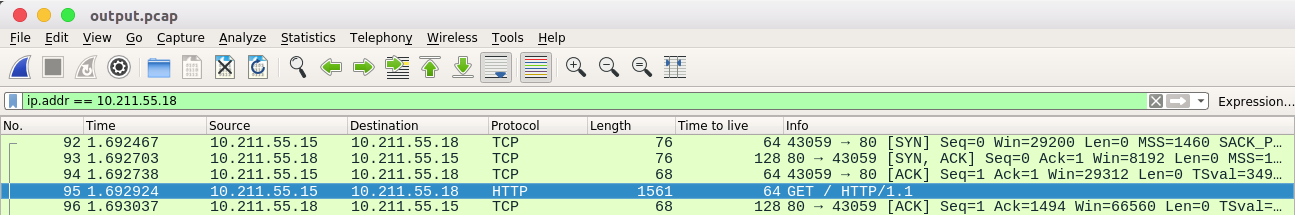
\includegraphics[width=.9\linewidth]{./images/wireshark-http.png}
    \caption{\label{fig:wireshark-http}
      Screenshot of Wireshark displaying the HTTP request made by exploit to the Windows server}
  \end{figure}
  \item In the GET request in Figure~\ref{fig:get-request}, the Authorization header contains the payload.
  \begin{figure}[htbp]
    \centering
    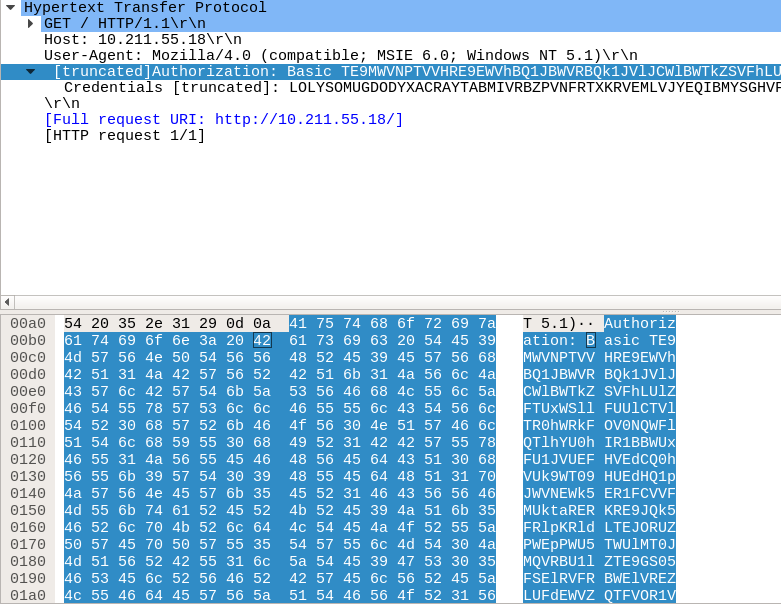
\includegraphics[width=.9\linewidth]{./images/get-request.png}
    \caption{\label{fig:get-request}
      Screenshot of Wireshark displaying the GET request and decoded payload}
  \end{figure}
  \item The payload is encoded to Base64 and excludes the bad characters so that Metasploit can
  determine the suitable payloads given the space available and OS of the victim.~\cite{metasploit} After
  decoding the payload, Figure~\ref{fig:get-request} shows that the payload contains random letters.
  \item 1012 bytes are required before overwriting the EIP. The EIP is overwritten with the target
  return address in little endian format.
  \item The target address is \verb|0x0040ae0f| in little endian format.
  \item The \verb|Space| variable specifies that theres is 600 bytes of space for the payload
  to reside in. If the payload is larger, it may cause corruption or truncation of the exploit.
  \item The exit function for the exploit is "thread". This affects the stability
  of the program after the exploit.
  \item CVE number: 2009-0183
  \item CVSS base score: 10.0 HIGH
  The score is high because the Free Download Manager is remotely exploitable, the access complexity is low,
  it does not require authentication, all system files are revealable, any file is modifiable, and
  the attacker can render the system unavailable.~\cite{cve}
  \item User: \verb|victimbox\class|
  \item Current Directory: \verb|C:\Program Files\Free Download Manager|
  \item OS: \verb|Windows 7 (6.1 Build 7601, Service Pack 1).|
  \item Current Process Name: \verb|fdmwi.exe|; Current PID: \verb|1096|
  \item Network Interfaces: 3; MAC Address of current connected interface: 00:1c:42:a9:26:bb
  \item Trying to acces the \verb|C:\Users\admin| directory, gives the following error message:
  \begin{minted}{bash}
  [-] stdapi_fs_chdir: Operation failed: Access is denied.
  \end{minted}
  \item Trying the \verb|getsystem| command gives the following error message. This is because the Meterpreter
  is not a SYSTEM user.
  \begin{minted}{bash}
  [-] priv_elevate_getsystem: Operation failed: Access is denied. The following was attempted:
  [-] Named Pipe Impersonation (In Memory/Admin)
  [-] Named Pipe Impersonation (Dropper/Admin)
  [-] Token Duplication (In Memory/Admin)
  \end{minted}
  \item User: \verb|NT AUTHORITY\SYSTEM|
  \item Exploit used: \verb|exploit/windows/local/ms13_081_track_popup_menu|
  \item Current Process Name: \verb|notepad.exe|; Current PID: 2100; Yes, it makes sense to 
  stay in this process to have elevated privelages.
  \item The hash for the admin user is: \verb|admin:1001:aad3b435b51404eeaad3b435b51404ee:7c098297bf993415889aad26435bb9cc:::|;
  The website CrackStation was used to decrypt the hashed password.~\cite{crack}
  \item Admin Password: \verb|iloveponies|
  \item Admin's Secret: \verb|i love lutefisk|
\end{enumerate}
\newpage
\section*{Conclusion}
\label{sec:conclusion}

\newpage
\nocite{*}
\bibliography{bibliography}
\bibliographystyle{ieeetr}
\end{document}
